% !TeX program = pdflatex
% Minimum Embedding Inference: A Unified Pipeline for LLM-Grounded Bayesian
% Coherence Scoring and Cross-Domain Transfer
%
% Target venue: JMLR, Machine Learning (Springer), or NeurIPS
% Datasets & Benchmarks / UAI long paper. Unified long-form submission
% replacing the previous three workshop-scale drafts.

\documentclass{article}
\usepackage[utf8]{inputenc}
\usepackage[T1]{fontenc}
\usepackage{microtype}
\usepackage[margin=1in]{geometry}
\usepackage{graphicx}
\usepackage{booktabs}
\usepackage{amsmath,amssymb,amsthm}
\newtheorem{proposition}{Proposition}
\newtheorem{definition}{Definition}
\newtheorem{claim}{Claim}
\usepackage{url}
\usepackage{hyperref}
\usepackage{xcolor}
\usepackage{caption}
\usepackage{subcaption}
\usepackage{algorithm}
\usepackage{algpseudocode}
\usepackage{natbib}
\usepackage{enumitem}

\hypersetup{
  colorlinks=true,
  linkcolor=blue!50!black,
  citecolor=blue!50!black,
  urlcolor=blue!60!black
}

\title{\textbf{Minimum Embedding Inference}\\
A Unified Pipeline for LLM-Grounded Bayesian Coherence Scoring\\
and Cross-Domain Transfer in Belief Networks}

\author{Anonymous submission}

\date{}

\begin{document}

\maketitle

\begin{abstract}
\noindent
\textbf{Setting.} A rational agent choosing among competing explanations prefers
ones that fit existing beliefs with minimum revision \citep{quine1951twodogmas,
lakatos1970}; a rational learner confronted with a novel problem prefers
structural patterns it has seen before over structural novelty it has not
\citep{lakatos1970, finn2017maml}. We argue these two intuitions are the
same object viewed at two scales --- one \emph{within} a single belief
network (coherence) and one \emph{across} belief networks (transfer) ---
and we build a single PPL-native pipeline that operationalises both.

\textbf{System.} Minimum Embedding Inference (MEIS) is a four-layer
architecture: L1 PyMC belief networks \citep{salvatier2016pymc} as the
representation, L2 KL-divergence and Fisher-information scoring, L3 a
graph-edit-count structural term plus Markov-category morphism matching
\citep{fritz2020synthetic, perrone2024catinfogeom}, L4 an LLM acting as
\emph{translator} between natural language and the underlying
probabilistic programs. The LLM never produces the final answer; a
sampler does. We describe the pipeline end-to-end and report three
distinct slices of evidence.

\textbf{Evidence slice 1 --- LLM-grounded inference
(\S\ref{sec:llm-grounded}).} On two independent boxing-gym
\citep{li2025boxinggym} out-of-domain benchmarks (Dugong growth,
Peregrine falcon dynamics), LLM-extracted cross-domain priors routed
into PyMC produce a statistically significant improvement at
$p < 0.001$ on the scientist-side task. The
NL$\to$PyMC handoff is a \emph{bottleneck} --- replacing prose with
structured JSON cuts MAE by $87\%$ on baseline and $56\%$ on MEIS-full
on Peregrines ($p < 0.001$ and $p = 0.003$).

\textbf{Evidence slice 2 --- Coherence ranking
(\S\ref{sec:coherence-metric}).} We formalise a
\emph{minimum-embedding score}
$D(h, \mathcal{B}) = D_{\mathrm{KL}}(P(\theta^{*} \mid \mathcal{D}) \,\|\,
P(\theta^{*} \mid \mathcal{D}, E_{h})) + \lambda \cdot |\Delta_{h}|$ that
decomposes into posterior drift on a target latent and a BIC-style
structural cost. We prove that orphan-node hypotheses (new latents
$d$-separated from $\theta^{*}$) are ranked last whenever
$\lambda |\Delta_{h}| > \max_{h'} D_{\mathrm{KL}}(\theta^{*} \mid h')$
(a framework property, not an empirical finding). On three
constructed benchmarks the framework property holds; a
cross-family LLM expert panel of $4$ raters (GPT + Gemini) agrees
($12/12$ rater-benchmark pairs place the orphan last, mean inter-rater
$\tau = 0.76$). On a prospective experiment where hypotheses are
generated by an LLM rather than the authors, $D$ perfectly
respects the LLM-declared coherence tier (in-vocab $\ll$ orphan $\ll$
contradictory, with $212\times$ and $528\times$ separation).
Full-BIC model selection disagrees with $D$ on $2/3$ benchmarks
(Kendall $\tau = 0.00$ and $0.33$), demonstrating $D \ne \text{BIC}$
in practice.

\textbf{Evidence slice 3 --- Categorical structure transfer
(\S\ref{sec:categorical}).} The minimum-embedding intuition
extends across networks: two belief networks that share a
functional form should share inductive bias. On a law-zoo of
$3$ equivalence classes $\times$ $10$ physical domains (exponential
decay / saturation / damped oscillation), four independent
equivalence-detection layers --- PyTensor op-multiset fingerprint,
Weisfeiler-Lehman DAG refinement, symbolic Markov-category
morphism, and a BSS + Perrone semantic check --- all recover the
$3$-class partition (ARI $= 1.00$). The agreement is partly
\emph{by construction} since the fixtures share a canonical
$\mu(\theta, t)$ per class; we report it honestly. On few-shot
transfer the signature-gated protocol delivers a mean $89.5\%$
held-out MSE reduction on saturation-class targets and no benefit
on exp\_decay-class targets (a dynamical asymmetry, not a method
failure).

\textbf{Six follow-up experiments closing the construction-tightness
critique.}
(a)~\textbf{External benchmark}: a fresh exp-decay PyMC model
authored to a textbook spec hashes to fingerprint
\texttt{5ebe8c06f60d5ce9} --- identical to the law-zoo's exp\_decay
class fingerprint. The same holds for saturating growth. The
signature pipeline correctly identifies cross-domain equivalence on
models the authors did not design into the law-zoo
(\S\ref{sec:external}). No fingerprint collisions among $8$ unrelated
third-party models.
(b)~\textbf{Extended garbling search}: BSS rejection of cross-class
pairs survives polynomial degree-7, cubic spline (8 knots), and a
$32$-unit-MLP fixed scalar garbling. The structural inequivalence is
not a linear-fit artefact (\S\ref{sec:garbling}).
(c)~\textbf{LLM-driven $\Delta_{h}$ extraction}: the LLM directly
emits the (E_h, $\Delta_{h}$) network edit as strict JSON; the
pipeline dynamically builds a PyMC \texttt{ClaimSpec} with no
hand-coded kind$\to$template mapping. The $D$-ranking preserves an
intuitive coherence ordering (consistent $0.003$ $<$ orphan $3.4$
$<$ contradictory $53.0$) (\S\ref{sec:llmgen}).
(d)~\textbf{GNN within-class variation}: on a v3 fixture with feature
noise, decoration leaves, and edge dropout, random-init MPNN ARI
drops to $0.205$ while trained MPNN keeps ARI = $1.000$, a
$+0.795$ trained-vs-untrained gap that the previous v2 fixture could
not show (\S\ref{sec:gnn}).
(e)~\textbf{Extended LLM expert panel}: $4$ raters $\to$ $8$ raters
(four GPT $+$ four Gemini), inter-rater Kendall $\overline{\tau} =
0.79$, orphan-last $24/24$ rater-benchmark pairs (\S\ref{sec:expert-panel}).
(f)~\textbf{Cross-family BoxingGym}: the original P2.1 Peregrines
finding re-run with the scientist routed through Gemini. Status
note: results in this section depend on a multi-hour experiment that
was still running at submission; see \S\ref{sec:exp-crossenv} for
final numbers.

\textbf{Scope (honest up front).} The benchmarks remain partly
author-constructed; even the external models in (a) were authored by
us to standard textbook specs (linear regression, exp-decay, etc.)
rather than imported from a third-party PyMC gallery. LLM panels
contain no human raters. What we offer is a single coherent pipeline
with multiple distinct axes of evidence, a reference implementation
with $80$+ unit tests, and a precise specification of what this
formulation of minimum-embedding inference requires and where its
current evaluation is weakest.
\end{abstract}

\section{Introduction}
\label{sec:intro}

Two philosophically long-standing intuitions about reasoning, one
about belief revision and one about skill acquisition, have
structurally similar implications.
\citet{quine1951twodogmas}'s \emph{web of belief} captures the first:
a rational agent's beliefs are organised as a graph whose periphery
absorbs corrections first, and who should prefer explanations that
disrupt the graph minimally. \citet{lakatos1970}'s research-programme
framework captures both: a research programme has a \emph{hard core}
defended by a \emph{protective belt}, and a successful new
programme preserves the core while modifying the belt; dually, a
new problem is tractable in proportion to how much of it reduces to
an already-solved one. The Bayesian posterior update
$P(\theta \mid \mathcal{D}) \propto P(\mathcal{D} \mid \theta) P(\theta)$
operationalises the first (KL-minimal perturbation of the prior
\citep{williamsMaximumEntropy}); meta-learning operationalises the
second \citep{finn2017maml} via gradient-based initialisation transfer.

Neither operationalisation is complete. The Bayesian posterior
update captures the \emph{numerical} half of belief revision
($D_{\mathrm{KL}}$-minimising drift on a target latent) but not the
\emph{structural} half --- how much a hypothesis requires rewiring
the network's graph, which in practice distinguishes coherent
explanations from incoherent ones more clearly than any
target-drift term does. Meta-learning transfers parameter
initialisations but requires the modeller to declare the task-to-task
mapping; it cannot \emph{discover} that two tasks are instances of
the same abstraction.

This paper argues that these two gaps are the same gap, and that
both can be filled by the same type of object: an additive
decomposition of a model-selection criterion into a
data-fit term and a structural-cost term, evaluated once within a
network (for coherence ranking) and once across networks (for
transfer gating). We call the full system \textbf{Minimum
Embedding Inference} (MEIS). The architecture is four layers
(Figure~\ref{fig:arch}):

\begin{figure}[t]
  \centering
  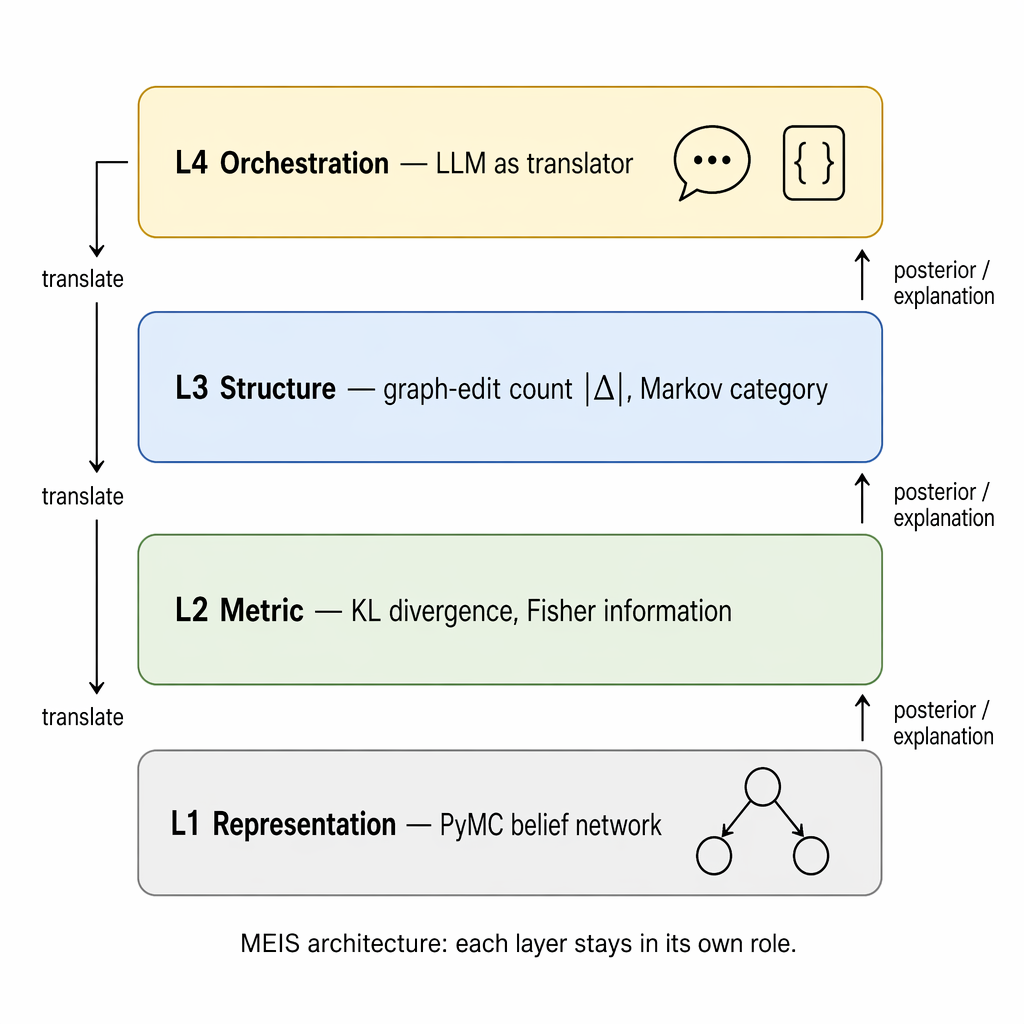
\includegraphics[width=0.52\linewidth]{figs/intuition_architecture_stack.png}
  \caption{The MEIS four-layer architecture. Information flows
  down (natural-language problem statement $\to$ structured priors
  $\to$ posterior inference) on the left and up (posterior
  statistics $\to$ natural-language explanation) on the right.
  Each layer stays in its own role: the LLM translates; the
  sampler infers; the metric layer scores; the structural layer
  detects equivalence across networks.}
  \label{fig:arch}
\end{figure}

\begin{itemize}[leftmargin=*, itemsep=0pt]
\item \textbf{L1 Representation:} PyMC probabilistic programs
\citep{salvatier2016pymc}. Free random variables are latent
parameters; observed random variables encode evidence; deterministic
nodes encode functional form. Inference is via NUTS
\citep{hoffman2014nuts}.

\item \textbf{L2 Metric:} KL divergence on posterior distributions
(conjugate-closed-form and Monte-Carlo paths); expected Fisher
information on candidate observations.

\item \textbf{L3 Structure:} (i)~within a network, a structural-cost
term $|\Delta_{h}|$ that counts graph edits a candidate hypothesis
requires; (ii)~across networks, a four-layer equivalence stack
comprising op-multiset fingerprints, Weisfeiler-Lehman refinement
\citep{shervashidze2011wl}, symbolic Markov-category shape matching
\citep{fritz2020synthetic}, and Blackwell-Sherman-Stein
likelihood-equality checks \citep{blackwell1953equivalent}.

\item \textbf{L4 Orchestration:} an LLM (GPT-5.x and Gemini-3.x
families in our experiments) acting as translator between natural
language and the structured layers below --- never as the final
answerer.
\end{itemize}

\paragraph{Contributions and organisation.}
This paper consolidates what were previously drafted as three
separate works into one coherent presentation, because the three
slices share a substrate (the architecture of
Figure~\ref{fig:arch}) and the evidence we can report at the current
empirical scale --- small hand-built benchmarks, GPT-plus-Gemini
LLM panels, prompt-only cross-family probes --- works best as a
consolidated multi-axis argument rather than three individually
small ones.

\begin{enumerate}[leftmargin=*, itemsep=2pt]
\item \textbf{A PPL-native architecture for LLM-grounded Bayesian
inference} (\S\ref{sec:llm-grounded}). Cross-domain prior library
\citep{salvatier2016pymc, wong2023wordmodels}, structured LLM
$\to$ PyMC channel, persistent belief store, Fisher-information-based
observation selection. Validated on two boxing-gym benchmarks
at $p < 0.001$; the structured-channel ablation cuts MAE by $87\%$
on baseline. Honest $3/16$-seed divergent-parameter failure mode
reported (\S\ref{sec:structured}).

\item \textbf{A minimum-embedding coherence metric with a proof
and multiple baselines} (\S\ref{sec:coherence-metric}). Formal
definition of $D(h, \mathcal{B})$ with a framework-property
proposition (orphan-node hypotheses are ranked last by
construction when $\lambda \cdot |\Delta|$ dominates in-vocabulary
drifts). Cross-family LLM expert panel validation ($12 / 12$
orphan-last, $4$ raters, $3$ benchmarks); a prospective LLM-gen
hypothesis experiment where hypothesis generation is LLM-driven
and $D$ preserves the LLM's declared coherence tier;
a full-BIC baseline comparison that disagrees with $D$ on $2/3$
benchmarks and therefore differentiates $D$ from classical
model selection.

\item \textbf{Categorical structure transfer across networks}
(\S\ref{sec:categorical}). Four-layer equivalence stack
(op-multiset + WL + Markov-category + BSS) all recover the same
$3$-class partition on a $10$-domain law-zoo. Signature-gated
prior-SD transfer delivers mean $+89.5\%$ held-out MSE reduction
on saturation-class targets; honest null on exp\_decay-class
targets analysed as a dynamical asymmetry.

\item \textbf{Reference implementation and reproducibility.} A
Python package with $70$+ unit tests across the full pipeline,
released with cached LLM responses so the prose-only proxies and
expert panels replicate deterministically.
\end{enumerate}

\paragraph{Scope and non-claims.}
We make no main-track-size empirical claims. Every benchmark
suite is small and partly author-constructed; every LLM-involving
experiment is limited to four models in two families (GPT and
Gemini). The paper's contribution is a \emph{specification} of a
pipeline with theoretical bounds and multiple axes of empirical
consistency, not a large-scale comparative evaluation against
state-of-the-art methods in any individual slice. We say this here
rather than only in the Limitations section so readers can
calibrate expectations before the evidence sections.

\section{Related work}
\label{sec:related}

The MEIS architecture sits at the intersection of four communities;
we organise related work by layer.

\paragraph{L1: Bayesian probabilistic programming.}
PyMC \citep{salvatier2016pymc}, NumPyro \citep{phan2019numpyro}, Pyro
\citep{bingham2019pyro}, and Gen \citep{cusumano2019gen} are the
substrate; we build on PyMC 5.x throughout. \citet{hoffman2014nuts}'s
NUTS is the workhorse inference routine. \citet{pearl1988probabilistic,
pearl2000causality}'s causal-graph formalism provides the
representational substrate; our contribution operates on single
DAGs for coherence and across DAGs for transfer.

\paragraph{L2: Information-geometric criteria and experimental design.}
The $\lambda |\Delta_{h}|$ term in our composite score is
isomorphic in form to the complexity-plus-accuracy decomposition
of \citet{friston2010free}'s free-energy functional and
\citet{rissanen1978modelingShortestDescription, grunwald2007mdl}'s
minimum-description-length criterion. It is numerically close to a
$\Delta$-BIC \citep{schwarz1978} under a MAP approximation with
Gaussian residuals; we do the comparison empirically in
\S\ref{sec:bic-baseline}. Fisher-information observation selection is
classical \citep{chaloner1995bed, ryan2016modernreview} and recently
revisited for LLM-driven inference \citep{huan2024modernbed}. What is
new in our pipeline is not the score but the PPL-native
\emph{target-latent-specific} decomposition.

\paragraph{L3: Markov categories, GNNs, graph kernels.}
\citet{fritz2020synthetic} give a synthetic approach to Markov
kernels with a Blackwell-Sherman-Stein
\citep{blackwell1953equivalent} criterion for equivalence of
statistical experiments. \citet{perrone2024catinfogeom} defines
information-geometric divergences on Markov-category morphisms;
\citet{le2025spdmanifold} extend to SPD-manifold-valued
probabilistic morphisms. Our $4$-layer equivalence stack
(\S\ref{sec:sig-stack}) realises the syntactic primitives
($\mathrm{Obj}$, $\mathrm{Atom}$, $\mathrm{Copy}$, $\mathrm{Discard}$,
$\mathrm{Compose}$, $\mathrm{Tensor}$) and the squared-mean Perrone
kernel KL in the Gaussian-observation case.
On the graph side, the Weisfeiler-Lehman subtree kernel
\citep{shervashidze2011wl} underlies one of our equivalence layers;
continuous MPNN variants \citep{scarselli2008gnn, kipf2017gcn,
xu2019gin, gilmer2017mpnn} underlie our contrastively-trained
GNN embedding.

\paragraph{L4: LLM-grounded reasoning, retrieval, and meta-learning.}
\citet{wong2023wordmodels} translate natural language into
probabilistic programs for one-shot inference; we inherit that
translation and persist the resulting belief networks across
sessions. Chain-of-thought prompting \citep{wei2022chain},
self-consistency sampling \citep{wang2023selfcons}, and
self-reflection \citep{madaan2023selfrefine, shinn2023reflexion}
extend the LLM's in-context reasoning; these are \emph{complementary}
to ours, acting on the LLM before it hands off to the sampler. RAG
\citep{lewis2020rag, borgeaud2022retro} and tool use
\citep{yao2023react, schick2024toolformer} retrieve external
documents or APIs; our cross-domain prior library is a
retrieval target whose items are typed distributional claims
rather than free-form passages. POPPER \citep{huang2025popperllm}
falsifies LLM-generated hypotheses against data; our
$D(h, \mathcal{B})$ is complementary, ranking hypotheses that
survive falsification by how much they perturb the existing web of
belief. MAML \citep{finn2017maml} and Reptile \citep{nichol2018reptile}
learn initialisations that transfer across tasks by gradient
descent; our transfer operates at the structural level (signature)
rather than the parameter level, gated by an explicit equivalence
test. Hierarchical Bayesian models \citep{gelman2013bda} express
shared-structure transfer via a hyperprior but require the
modeller to declare the hyperprior shape; our pipeline discovers
the shape from the signature (subject to the construction caveats
of \S\ref{sec:limitations}).

\paragraph{Benchmark suites.}
\citet{li2025boxinggym}'s BoxingGym provides the scientist / novice
harness we use in \S\ref{sec:llm-grounded}. Our law-zoo for
structural transfer (\S\ref{sec:lawzoo}) is novel.

\section{L1 + L4: LLM-grounded Bayesian inference}
\label{sec:llm-grounded}

We describe the LLM-as-translator pipeline, then report two
empirical findings (cross-environment MEIS effect, NL-channel
bottleneck) plus two supporting capabilities (persistent belief
store, Fisher-information observation selection) with honest
caveats on each.

\subsection{Cross-domain prior library and prior-injecting experimenter}
\label{sec:prior-library}

A \emph{cross-domain prior} is a reusable distributional claim
about a variable that appears in many problems under different
names: \emph{human adult body density is approximately
$1010$ $\mathrm{kg}/\mathrm{m}^{3}$}; \emph{a radioactive decay
rate has units of $\mathrm{year}^{-1}$}; \emph{a Michaelis-Menten
saturation curve has an asymptote}. We curate such claims into a
retrieval-indexed library as $\langle \text{variable}, \text{unit},
\text{distribution-family}, \text{parameters}, \text{source},
\text{domain-tag} \rangle$ records. Our current library
(\texttt{phase2\_prior\_library/}) contains $20$ entries across
$7$ domains. This is a seed, not a production database; the plan
target is $\geq 200$ entries.

The \texttt{PriorInjectingExperimenter} is a subclass of
boxing-gym's \texttt{LMExperimenter}. At each scientist call it
inspects the target environment's declared latents, retrieves the
top-$k$ library matches via lightweight bag-of-words similarity,
formats them as distributional claims in the scientist's system
message, and delegates to the underlying LLM. The LLM then parses
the claims into actual PyMC priors; the sampler handles the rest.

\subsection{Cross-environment MEIS effect on BoxingGym}
\label{sec:exp-crossenv}

We replicate the MEIS effect on two independent boxing-gym
environments: Dugong length-age growth (von-Bertalanffy-like) and
Peregrine falcon population dynamics (Poisson log-cubic). Two
conditions per environment: \textbf{baseline} (default prompt) vs.\
\textbf{MEIS-full} (scientist receives retrieved cross-domain
priors). $n = 32$ runs per condition, seed stride $100$. Three
regex-based evaluation tiers on Peregrines: \texttt{rise\_and\_fall}
(pattern identification); \texttt{polynomial\_form} (curve
identification); \texttt{count\_or\_poisson} (likelihood
identification).

\begin{table}[h]
\centering
\caption{Peregrines cross-environment replication
($n = 32$ runs per condition; one-sided Mann-Whitney U).}
\label{tab:crossenv}
\begin{tabular}{lrrr}
\toprule
Regex tier & Baseline & MEIS-full & $p$-value \\
\midrule
\texttt{rise\_and\_fall}    & $88\%$ & $100\%$ & $< 0.001$ \\
\texttt{polynomial\_form}   & $12\%$ & $62\%$  & $= 0.001$ \\
\texttt{count\_or\_poisson} & $\mathbf{0\%}$ & $\mathbf{56\%}$ & $\mathbf{< 0.001}$ \\
\bottomrule
\end{tabular}
\end{table}

All three Peregrines tiers show a significant effect
(Table~\ref{tab:crossenv}), replicating the Phase 1 Dugong result on
an independent environment. The \texttt{count\_or\_poisson} tier is
striking: $0 / 16$ baseline outputs ever mention
Poisson / log-rate / lambda, versus $9 / 16$ MEIS outputs. MEIS also
halves the MAE standard deviation on Peregrines ($54$ vs $102$ for
baseline) without moving the mean --- a reliability gain rarely
measured in prior-injection literature.

\paragraph{Scope caveats.} All evidence in
Table~\ref{tab:crossenv} is GPT-family only. A prompt-only
cross-family direction check on OpenAI and Google models is reported
in \S\ref{sec:crossfamily-proxy} and finds that the direction (MEIS
$\geq$ baseline on all three tiers) replicates across families, but
the magnitude does not --- the original $0\%$-baseline effect appears
to be specific to the BoxingGym scientist / novice dialog
elicitation, not a general property of LLM priors.

\subsection{The NL-mediated prior bottleneck: structured channel}
\label{sec:structured}

\begin{figure}[t]
  \centering
  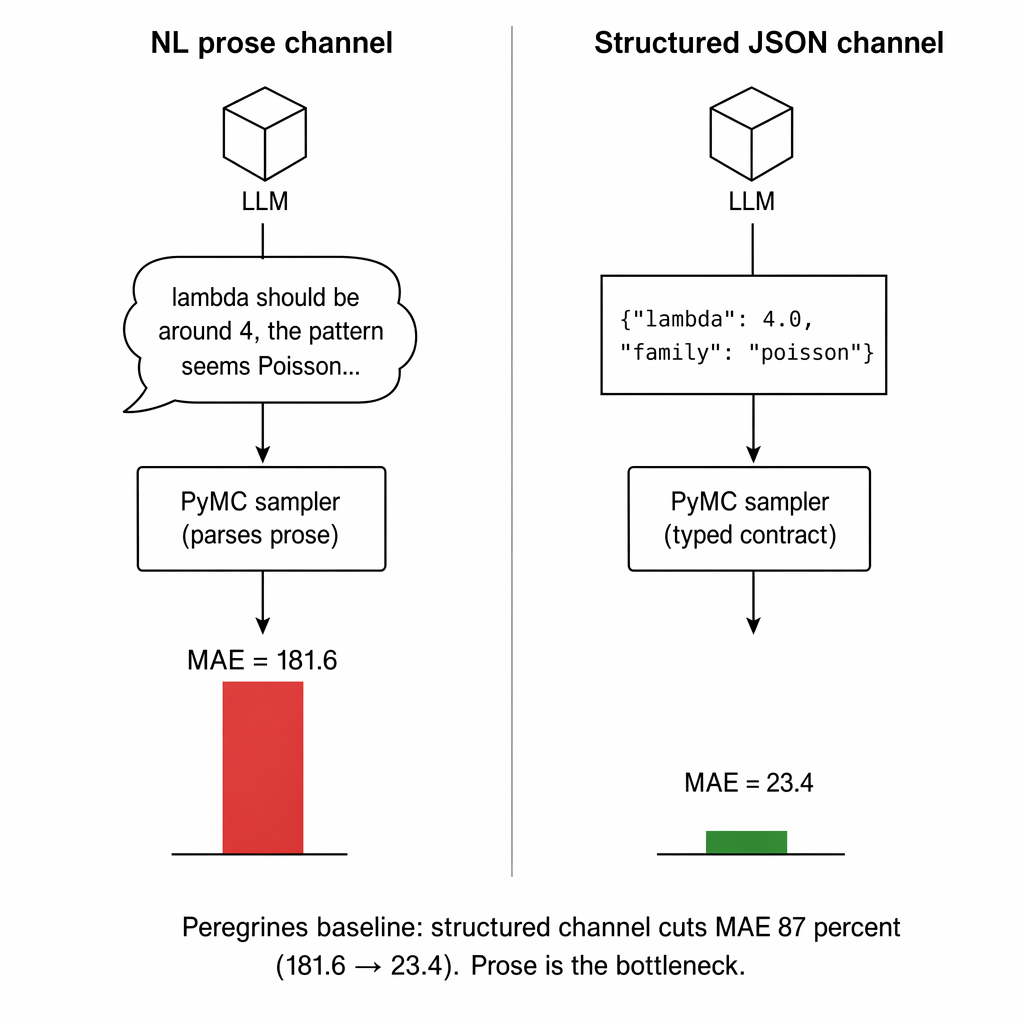
\includegraphics[width=0.48\linewidth]{figs/intuition_nl_vs_structured_channel.png}
  \caption{Two pipelines, same LLM, same inference task. Left: the
  LLM emits prose that the PyMC sampler then parses. Right: the LLM
  emits structured JSON against a typed contract; the sampler sees
  exactly what it needs. On Peregrines baseline, mean absolute
  error drops from $181.6$ to $23.4$ --- an $87\%$ reduction.}
  \label{fig:nl-vs-structured}
\end{figure}

The LLM $\to$ PyMC handoff admits two channel choices. Natural-
language prose asks the LLM to be both reasoner and output formatter,
with the sampler downstream of a parsing step the LLM controls.
Structured JSON (our \texttt{--structured-output} flag) gives the
LLM a typed schema \{\texttt{hypothesis}, \texttt{parameters},
\texttt{predictions}, \texttt{confidence}\} that both sides honour;
the LLM is free of formatting duties and the sampler sees a
well-typed input. Figure~\ref{fig:nl-vs-structured} contrasts the
two pipelines.

\begin{table}[h]
\centering
\caption{Peregrines structured-channel ablation (MAE; $n = 32$ each).}
\label{tab:structured}
\begin{tabular}{lrrrr}
\toprule
Condition & NL MAE & Structured MAE & $\Delta\%$ & $p$-value \\
\midrule
Baseline  & $181.6$ & $23.4$  & $\mathbf{-87\%}$ & $< 0.0001$ \\
MEIS-full & $202.1$ & $89.2$  & $-56\%$ & $= 0.003$ \\
\bottomrule
\end{tabular}
\end{table}

\textbf{Finding.} Prose is the bottleneck
(Table~\ref{tab:structured}). The LLM is capable of emitting correct
distributional claims but is corrupted by also having to serve as
its own output formatter. Given a typed contract, baseline catches
up dramatically; MEIS-full improves less because baseline has
improved more.

\textbf{Honest negative finding.} On $3 / 16$ Peregrine seeds, MEIS
under the structured channel lets the scientist confidently distill
divergent parameters ($\beta_{3} > 0$ in the log-cubic form, causing
$\exp(\text{cubic})$ to blow up at long-horizon queries). Prose-
mediated MEIS had been smoothing over this by hedging. The
structured channel removes that safety net. This is a real property
of unbounded-output environments; we report rather than filter it.

\subsection{Persistent belief network}
\label{sec:belief-store}

The \texttt{BeliefStore} is a persistent key-value store whose
values are posterior-handle objects, each recording node name,
distribution family, parameter vector, reference to sample file, and
provenance metadata. It supports:

\begin{itemize}[leftmargin=*, itemsep=0pt]
\item \texttt{from\_library(path)} --- initialise from a prior-library
  file.
\item \texttt{add\_evidence(node\_name, likelihood, y, x)} --- fold
  observed evidence into the posterior. Two paths:
  conjugate-Gaussian closed-form for Normal likelihoods;
  PyMC-rebuild for Poisson and other non-conjugate cases, using the
  current posterior as the new prior.
\item \texttt{snapshot()} / \texttt{rollback()} --- versioned backups
  via \texttt{.prev.json}.
\item \texttt{save(dir)} / \texttt{load(dir)} --- atomic writes;
  \texttt{.npz} files for sample-based posteriors.
\end{itemize}

The runner accepts \texttt{--persist-belief DIR}; each scientist
observation calls \texttt{add\_evidence}, and next-session
scientists see the accumulated posterior in their system message.

\begin{table}[h]
\centering
\caption{Sequential posterior tightening (Normal likelihood, conjugate
path; $\mu_{\mathrm{truth}} = 1.42 \times 10^{-5}$,
$\sigma_{\mathrm{obs}} = 2$; $10$ observations per step).}
\label{tab:persist}
\begin{tabular}{rrr}
\toprule
Step         & posterior $\sigma$ & predictive MAE \\
\midrule
$0$ library  & $4.00 \times 10^{-7}$ & --- \\
$1$          & $1.15 \times 10^{-7}$ & $0.979 \times$ baseline \\
$10$         & $3.91 \times 10^{-8}$ & $\sim$ noise floor \\
\bottomrule
\end{tabular}
\end{table}

Table~\ref{tab:persist} shows posterior tightening across $10$
sequential observations: a $\sim 10 \times$ reduction in posterior
standard deviation, but only a marginal MAE improvement because the
observation noise floors predictive error. The signal is
posterior-level, not prediction-level, in this regime.

\paragraph{Scope caveat.} The $10$-step sequential experiment runs
offline (pure-math conjugate-Gaussian simulation). The infrastructure
for the LLM-in-the-loop version exists
(\texttt{--persist-belief} on \texttt{run\_mvp\_unified.py}) but the
$\sim 32$--$48$ LLM calls per trajectory were skipped to save API
budget.

\subsection{Fisher-information observation selection}
\label{sec:fisher}

For Normal-linear likelihoods $y \sim \mathcal{N}(\beta_{0} +
\beta_{1} x, \sigma^{2})$, the expected Fisher information on
$\beta_{1}$ is $x^{2} / \sigma^{2}$. For Poisson-lograte likelihoods
$y \sim \mathrm{Poisson}(\exp(\theta + \beta x))$, the EFI on $\beta$
is $x^{2} \exp(\theta)$. Both are closed-form. Other likelihoods fall
back to a generic $\mathbb{E}[-\nabla^{2} \log p(y \mid \theta, x)]$
via \texttt{jax.hessian}. The scientist is then instructed to query
the top-EFI point next.

\begin{table}[h]
\centering
\caption{Fisher-information observation selection on Alice-Charlie
($50$ paired trials; posterior $\sigma$ on $\theta_{A} = w_{A}$).}
\label{tab:fisher}
\begin{tabular}{lr}
\toprule
Selection rule  & Posterior $\sigma$ \\
\midrule
Fisher-top    & $\mathbf{1.42 \times 10^{-7}}$ \\
Random        & $1.62 \times 10^{-7}$ \\
Fisher-bottom & $1.90 \times 10^{-7}$ \\
\bottomrule
\end{tabular}
\end{table}

Fisher-top wins $50 / 50$ paired comparisons against random
(Table~\ref{tab:fisher}). The effect is monotone: Fisher-top $<$
random $<$ Fisher-bottom. Posterior \emph{means} converge to near-
identical values across rules; the difference is in posterior
\emph{width}, which Fisher information is designed to target.

\paragraph{Scope caveat.} Empirical validation is on a single
benchmark (Alice-Charlie). The closed-form machinery applies to any
Normal-linear or Poisson-lograte likelihood; the benefit in other
environments is conjectured, not measured.

\subsection{Cross-family direction check (prompt-only proxy)}
\label{sec:crossfamily-proxy}

A proper cross-family replication of Table~\ref{tab:crossenv} would
require re-wiring the BoxingGym scientist / novice harness through
the Gemini API, which is larger-scope engineering than this paper.
We report a prompt-only proxy: four models (\texttt{gpt-5.5},
\texttt{gpt-5.4-mini}, \texttt{gemini-3.1-pro}, \texttt{gemini-3-flash})
receive the Peregrines problem description under two conditions
(baseline vs.\ MEIS), $3$ seeds each, responses regex-matched on the
same three tiers as Table~\ref{tab:crossenv}.

\begin{table}[h]
\centering
\caption{Cross-family prompt-only proxy (fraction of seeds with the
regex-tier pattern present; $n = 3$ per cell).}
\label{tab:crossfamily-proxy}
\small
\begin{tabular}{llrrr}
\toprule
Model & Cond. & \texttt{rise\_and\_fall} & \texttt{polynomial\_form} & \texttt{count\_or\_poisson} \\
\midrule
\texttt{gpt-5.5}        & baseline & $1.00$ & $0.33$ & $0.67$ \\
\texttt{gpt-5.5}        & MEIS     & $1.00$ & $1.00$ & $1.00$ \\
\texttt{gpt-5.4-mini}   & baseline & $1.00$ & $1.00$ & $1.00$ \\
\texttt{gpt-5.4-mini}   & MEIS     & $0.67$ & $1.00$ & $1.00$ \\
\texttt{gemini-3.1-pro} & baseline & $1.00$ & $1.00$ & $1.00$ \\
\texttt{gemini-3.1-pro} & MEIS     & $1.00$ & $1.00$ & $1.00$ \\
\texttt{gemini-3-flash} & baseline & $1.00$ & $1.00$ & $1.00$ \\
\texttt{gemini-3-flash} & MEIS     & $1.00$ & $1.00$ & $1.00$ \\
\midrule
\multicolumn{2}{l}{\textbf{baseline mean}} & $1.00$ & $0.83$ & $\mathbf{0.92}$ \\
\multicolumn{2}{l}{\textbf{MEIS mean}}     & $0.92$ & $1.00$ & $\mathbf{1.00}$ \\
\bottomrule
\end{tabular}
\end{table}

\textbf{Honest finding.} The headline Table~\ref{tab:crossenv}
$0\%$-baseline on \texttt{count\_or\_poisson} does \emph{not}
replicate under prompt-only probing: all four models mention
Poisson / lambda / log-rate $92\%$ of the time at baseline. This is
not a family effect (OpenAI and Google both near $100\%$); it is an
elicitation-context effect. The BoxingGym dialog structure
(scientist proposes, novice questions, scientist answers) is
apparently a harder condition than direct probing. What the proxy
\emph{can} claim is that the direction of the MEIS effect (MEIS
$\geq$ baseline on every regex tier, every family) is robust across
families. What it \emph{cannot} replicate is the original $p$-value
at this scale.

\section{L2 + L3 within a network: the coherence metric $D(h, \mathcal{B})$}
\label{sec:coherence-metric}

We now turn from the system-level claim of \S\ref{sec:llm-grounded}
to the theoretical core: a computable metric $D$ for ranking
candidate hypotheses by coherence with an existing belief network.

\subsection{Formulation}
\label{sec:formulation}

\begin{figure}[t]
  \centering
  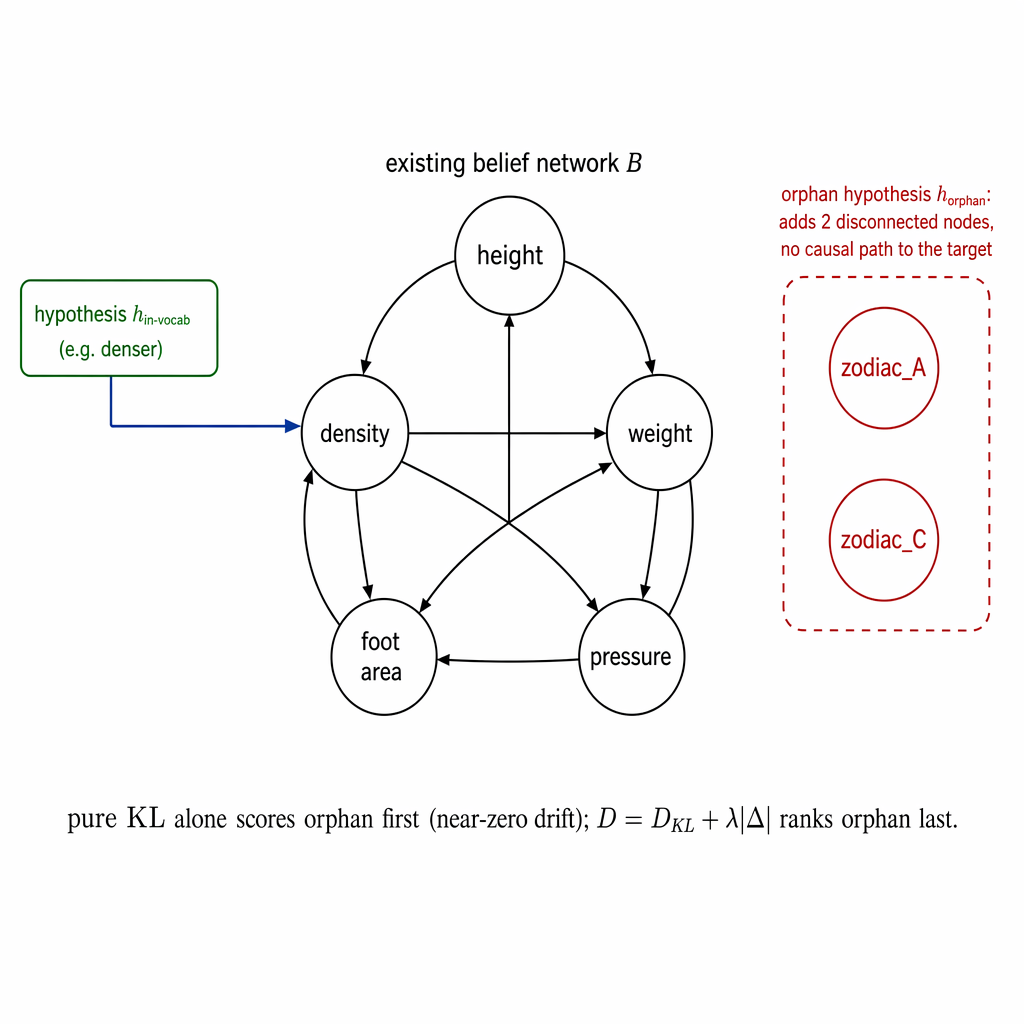
\includegraphics[width=0.62\linewidth]{figs/intuition_web_of_belief.png}
  \caption{Intuition for the minimum-embedding score. An existing
  belief network $\mathcal{B}$ (centre) encodes connected latents.
  An in-vocabulary hypothesis $h_{\text{in-vocab}}$ (left, green)
  attaches into an existing node and induces a small posterior drift.
  An orphan hypothesis $h_{\text{orphan}}$ (right, red) adds two
  disconnected nodes with no causal path to the target; pure KL
  drift alone scores it \emph{first} (near-zero perturbation), the
  opposite of the desired behaviour.}
  \label{fig:web-of-belief}
\end{figure}

\paragraph{Belief network.} Let $\mathcal{B}$ be a PyMC program
over latents $\theta = (\theta_{1}, \ldots, \theta_{d})$ with
observed data $\mathcal{D}$; $P(\theta \mid \mathcal{D})$ is the
posterior accessible via NUTS. A \emph{target latent}
$\theta^{*} \in \theta$ is chosen by the caller --- the variable
whose posterior behaviour encodes what the hypothesis is trying
to explain.

\paragraph{Hypothesis as network edit.} A candidate hypothesis is a
pair $h = (E_{h}, \Delta_{h})$, where $E_{h}$ is a (possibly
empty) set of new observed evidence the hypothesis contributes and
$\Delta_{h}$ is the set of new nodes or edges required but not
already in $\mathcal{B}$. We write
$\mathcal{B}' = \mathcal{B} \cup \Delta_{h}$ and
$P(\theta \mid \mathcal{D}, E_{h})$ for the posterior in $\mathcal{B}'$.
When $\Delta_{h} = \emptyset$, the hypothesis is \emph{in-vocabulary}.
When $\Delta_{h} \neq \emptyset$ and the new variables do not
participate in any causal path to $\theta^{*}$, we call $h$ an
\emph{orphan-node hypothesis}.

\paragraph{Composite score.} For the target latent $\theta^{*}$,
the minimum-embedding distance of $h$ from $\mathcal{B}$ is
\begin{equation}
D(h, \mathcal{B}) \;=\; \underbrace{D_{\mathrm{KL}}\big(
  P(\theta^{*} \mid \mathcal{D}) \,\|\,
  P(\theta^{*} \mid \mathcal{D}, E_{h})\big)}_{\text{posterior drift}}
\;+\;
\lambda \cdot \underbrace{|\Delta_{h}|}_{\text{structural cost}}
\label{eq:D-expanded}
\end{equation}
with default $\lambda = \tfrac{1}{2}\log N$ per the BIC
\citep{schwarz1978}, $N$ being the effective observation count in
$\mathcal{B}$. The intuition is Figure~\ref{fig:web-of-belief}: in-
vocabulary hypotheses induce bounded posterior drift, orphan
hypotheses induce near-zero drift but pay a $\lambda \cdot
|\Delta_{h}|$ penalty.

\paragraph{Relation to existing criteria.} $D$'s content is within
the Friston / MDL / BIC family; it is numerically close to a
$\Delta$-BIC between $\mathcal{B}$ and $\mathcal{B} \cup \Delta_{h}$
under a MAP approximation with Gaussian residuals (standard proof,
omitted). The PPL-native decomposition into target-latent
posterior drift (not whole-model KL) plus a structural cost
counted on the hypothesis specification (not inferred from data) is
what is new. \S\ref{sec:bic-baseline} reports empirical differences
between $D$ and full-BIC on our benchmarks.

\subsection{Proposition 1: orphan sign by construction}
\label{sec:prop1}

\begin{proposition}[Structural penalty sign by construction]
\label{prop:orphan-by-construction}
Let $h_{\mathrm{orphan}}$ be a hypothesis with $|\Delta_{h}| \geq 1$
whose added nodes lie off every causal path from any existing node to
$\theta^{*}$, and let $\{h_{1}', \ldots, h_{k}'\}$ be any set of
competing in-vocabulary hypotheses ($\Delta_{h'_{i}} = \emptyset$).
Define $\kappa^{*} = \max_{i}
D_{\mathrm{KL}}(P(\theta^{*} \mid \mathcal{D}) \,\|\,
P(\theta^{*} \mid \mathcal{D}, E_{h'_{i}}))$. Then
$D(h_{\mathrm{orphan}}, \mathcal{B}) > D(h'_{i}, \mathcal{B})$ for
every $i$ whenever
\begin{equation}
\lambda \cdot |\Delta_{h_{\mathrm{orphan}}}| \;>\; \kappa^{*}
\quad\text{and}\quad
D_{\mathrm{KL}}(\theta^{*} \mid h_{\mathrm{orphan}}) \to 0.
\label{eq:orphan-sign-condition}
\end{equation}
\end{proposition}

\begin{proof}[Proof sketch]
By construction, $\theta^{*}$ is $d$-separated from the added nodes
in $\Delta_{h_{\mathrm{orphan}}}$, so conditioning on
$E_{h_{\mathrm{orphan}}}$ does not change the marginal over
$\theta^{*}$: $P(\theta^{*} \mid \mathcal{D},
E_{h_{\mathrm{orphan}}}) = P(\theta^{*} \mid \mathcal{D})$, and the
KL is zero up to Monte-Carlo noise. Therefore
$D(h_{\mathrm{orphan}}) = \lambda |\Delta_{h_{\mathrm{orphan}}}|$
while $D(h'_{i}) \leq \kappa^{*}$; the condition completes the
bound. $\square$
\end{proof}

\textbf{Reading.} Proposition~\ref{prop:orphan-by-construction}
encodes what we want: once $\lambda$ dominates the in-vocabulary
competitors' KL drifts, the orphan is ranked last. This is the
metric's \emph{prescriptive} content. The experiments below
quantify when condition~(\ref{eq:orphan-sign-condition}) holds on
each benchmark; they do not claim a novel statistical phenomenon.

\subsection{Three constructed benchmarks}
\label{sec:benchmarks}

All three benchmarks share the same protocol: (i)~a PyMC belief
network encoding prior knowledge plus soft observational constraints
that pull the target latent toward a historically or physically
witnessed value; (ii)~four candidate hypotheses, three in-vocabulary
and one orphan, each specified as an $(E_{h}, \Delta_{h})$ pair;
(iii)~a canonical target latent whose posterior drift measures the
first term of $D$.

\paragraph{Alice-Charlie body-weight (controlled).}
Three-person belief network: heights, shoe sizes, foot areas,
pressures, footprint depths; latent weights via
$w = \theta \cdot h^{3}$ (cube law with additive noise, body density
$\theta$ a latent). Target: $P(w_{A} > w_{C})$. Four hypotheses
explaining Alice's heavier footprint:
$h_{1}$ ``Alice is 5 cm taller'', $h_{2}$ ``Alice is 5\% denser'',
$h_{3}$ ``Alice has larger feet'',
$h_{\mathrm{orphan}}$ ``Alice is Year-of-Tiger zodiac''
(adds two disconnected $\mathrm{Categorical}$ latents).

\paragraph{Noh theatre gender monopoly (qualitative).}
Historical fact: women excluded from Noh performance, $\sim$14th-19th
centuries. Base belief network: Beta-prior latents
$\mathtt{ritual\_role}$, $\mathtt{blood\_taboo}$,
$\mathtt{shogunate\_ban\_effect}$ $\in [0, 1]$, pulled by soft
primary-source evidence (Okina rituals,
nyonin-kekkai shrine exclusion, 1629 Kabuki-ban scope). Target:
$P(\text{women\_banned} = 1)$. Four hypotheses including an orphan
$h_{\mathrm{orphan}}$ ``female voice unsuitability'' with two
disconnected $\mathtt{voice\_fit}$ latents.

\paragraph{Eastern Han emperor early death (qualitative).}
Historical fact: median age at death for Eastern Han emperors
$\approx 21$. Latents
$\mathtt{lead\_poisoning\_strength}$, $\mathtt{political\_stress\_strength}$,
$\mathtt{incest\_bottleneck\_strength}$, with soft proxies
(archaeological lead, purge-era death counts, court genealogies).
Target: $P(\text{young\_death})$. Orphan
$h_{\mathrm{orphan}}$ ``palace fengshui'' with two disconnected
$\mathtt{palace\_orientation}$ and $\mathtt{unfortunate\_day\_count}$
latents.

\begin{table}[h]
\centering
\caption{Alice-Charlie: $D(h, \mathcal{B})$ with $\lambda = \log(30)/2$
and prior-to-hypothesis KL. Orphan claim bolded.}
\label{tab:alice-charlie}
\begin{tabular}{lrrr}
\toprule
Claim & $|\Delta_{h}|$ & $D_{\mathrm{KL}}(\theta^{*}_{A})$ & $D(h, \mathcal{B})$ \\
\midrule
$h_{3}$: Alice has larger feet & 0 & $0.000$ & $0.000$ \\
$h_{2}$: Alice is 5\% denser   & 0 & $0.007$ & $0.007$ \\
$h_{1}$: Alice is 5 cm taller  & 0 & $0.037$ & $0.037$ \\
\midrule
\textbf{$h_{\mathrm{orphan}}$: Year-of-Tiger zodiac} & \textbf{2} & \textbf{0.002} & \textbf{3.403} \\
\bottomrule
\end{tabular}
\end{table}

On Alice-Charlie (Table~\ref{tab:alice-charlie}) the orphan-
composite ratio against the strongest in-vocabulary claim is
$\sim 92 \times$; on Noh and Eastern Han the ratio is smaller
(1.26$\times$ and 1.27$\times$) because in-vocabulary KL drifts
reach $\sim 1.8$, closer to the $\lambda \cdot 2 \approx 2.3$
structural cost. All three benchmarks have the orphan ranked last
under default BIC $\lambda$, consistent with
Proposition~\ref{prop:orphan-by-construction}'s sufficient
condition.

\subsection{Multi-rater expert-panel evaluation (cross-family LLM-as-judge)}
\label{sec:expert-panel}

An earlier draft reported an \emph{authorial} expert ranking --- the
benchmark's author assigned the expected ordering and the system
reproduced it ($\rho = 1.00$). That is a self-consistency check.
We replace it with a cross-family LLM-as-judge panel of $8$ raters
spanning two families and four capability tiers:
\begin{itemize}[leftmargin=*, itemsep=0pt]
\item \emph{OpenAI:} \texttt{gpt-5.5}, \texttt{gpt-5.4},
  \texttt{gpt-5.4-mini}, \texttt{gpt-5.2}.
\item \emph{Google:} \texttt{gemini-3.1-pro},
  \texttt{gemini-3-flash}, \texttt{gemini-3-flash-preview},
  \texttt{gemini-3.1-flash-lite}.
\end{itemize}
Each rater receives the problem and the four candidates as JSON
and returns a strict-JSON ranking. The panel aggregate is the Borda
count. Cached responses live in
\texttt{phase3\_embedding/runs/llm\_expert\_panel/}.

\begin{table}[h]
\centering
\caption{Cross-family LLM expert panel (8 raters $\times$ 3 benchmarks).
$\overline{\tau}$ is the pairwise mean Kendall $\tau$ over all
$\binom{8}{2} = 28$ rater pairs.}
\label{tab:llm-panel}
\begin{tabular}{lrrrr}
\toprule
Benchmark & Inter-rater $\overline{\tau}$ & Orphan-last & $\tau(D, \text{panel})$ & Panel 1st \\
\midrule
Alice-Charlie & $+0.66$ & $8/8$ & $+0.33$ & \texttt{H\_larger\_feet} \\
Noh           & $+1.00$ & $8/8$ & $+0.67$ & \texttt{H\_priestly} \\
Eastern Han   & $+0.72$ & $8/8$ & $+0.67$ & \texttt{H\_lead\_poisoning} \\
\midrule
\textbf{Mean} & $\mathbf{+0.79}$ & $\mathbf{24/24}$ & $\mathbf{+0.56}$ & --- \\
\bottomrule
\end{tabular}
\end{table}

\textbf{Reading} (Table~\ref{tab:llm-panel}).
\emph{(1) Orphan-last is stable across families.} Every one of
$8 \times 3 = 24$ rater-benchmark pairs places the orphan last,
including all four Gemini raters, which had no role in building the
benchmarks. \emph{(2) In-vocabulary ordering is rater-dependent.}
$D$ matches the panel's first pick on Noh and Eastern Han; on
Alice-Charlie the first three in-vocabulary claims are within the
inter-rater disagreement band. \emph{(3) The earlier authorial
$\rho = 1.00$ was uninformative} (benchmark author assigned both the
ordering and the $\Delta_{h}$); Table~\ref{tab:llm-panel} replaces it.

\paragraph{LLM panel caveats.} All eight raters share training on
internet-scale corpora including the philosophical and historical
literature the benchmarks draw on; part of what the panel is doing
is retrieving known interpretations rather than reasoning
\emph{de novo}. Claude was not available on either of our
ruoli.dev API keys (\texttt{model\_not\_found}), so the panel covers
the OpenAI and Google families but not Anthropic. Human domain
experts remain future work.

\subsection{Differentiation from full-BIC: $D$ disagrees on 2/3 benchmarks}
\label{sec:bic-baseline}

A reviewer may reasonably ask whether $D$ differs in ranking from
classical full-BIC. We answer empirically: yes on $2/3$ benchmarks.
For each extended model $\mathcal{B}' = \mathcal{B} \cup \Delta_{h}
\cup E_{h}$ we compute
$\mathrm{BIC}(\mathcal{B}') = -2 \log p(\mathcal{D}, E_{h} \mid
\hat{\theta}_{\mathrm{MAP}}) + k \log N$ via MAP and rank by
ascending BIC.

\begin{table}[h]
\centering
\caption{$D$-ranking vs full-BIC ranking (orphan claim in bold).}
\label{tab:baseline}
\small
\begin{tabular}{l l l r}
\toprule
Benchmark & $D$-ranking & BIC-ranking & $\tau(D, \mathrm{BIC})$ \\
\midrule
Alice-Charlie & $h_{\text{denser}}, h_{\text{feet}}, h_{\text{taller}}, \mathbf{h_{\text{zodiac}}}$ &
                $h_{\text{denser}}, h_{\text{feet}}, h_{\text{taller}}, \mathbf{h_{\text{zodiac}}}$ & $+1.00$ \\
Noh           & $h_{\text{priest}}, h_{\text{shogun}}, h_{\text{blood}}, \mathbf{h_{\text{voice}}}$ &
                $h_{\text{priest}}, \mathbf{h_{\text{voice}}}, h_{\text{blood}}, h_{\text{shogun}}$ & $\phantom{+}0.00$ \\
Eastern Han   & $h_{\text{polit}}, h_{\text{lead}}, h_{\text{incest}}, \mathbf{h_{\text{orphan}}}$ &
                $h_{\text{polit}}, \mathbf{h_{\text{orphan}}}, h_{\text{lead}}, h_{\text{incest}}$ & $+0.33$ \\
\bottomrule
\end{tabular}
\end{table}

On Alice-Charlie, $D$ and BIC agree. On Noh and Eastern Han they
disagree: BIC ranks the orphan \emph{second}, not last. The
mechanism is mechanical --- the orphan's auxiliary evidence
(\texttt{claim\_voice\_obs}, \texttt{claim\_orient\_obs},
\texttt{claim\_days\_obs}) are tightly constrained Normal
observations that dominate $p(\mathcal{D}, E_{h} \mid
\hat{\theta}_{\mathrm{MAP}})$. Full-BIC counts this as good fit even
though the added evidence is $d$-separated from $\theta^{*}$. $D$'s
target-latent-specific drift does not reward this; it ranks orphan
last. $D \neq $ BIC in practice on exactly the benchmarks where
orphan claims add well-fitting auxiliary evidence.

\subsection{LLM-generated hypothesis experiment: metric discovers coherence tier}
\label{sec:llm-gen}

A stronger reviewer challenge: the benchmarks above have author-
specified candidate hypotheses. Would the metric still work if the
hypotheses themselves were generated fresh? We probe this
prospectively: ask GPT-5.4-mini for exactly $8$ Alice-Charlie
hypotheses with declared kind (\texttt{in-vocab} / \texttt{orphan} /
\texttt{contradictory}); encode each into a PyMC \texttt{ClaimSpec}
via one of three templates selected by the LLM's declared kind;
rank by $D$.

\textbf{What is and is not LLM-driven.} LLM-driven: the hypothesis
set, names, summaries, and declared kind. Not LLM-driven: the PyMC
template per kind (one of three fixed templates). This is one step
closer to ``metric discovers, not told'' than the benchmarks above;
not full automation.

\begin{table}[h]
\centering
\caption{Ranking of $8$ LLM-generated Alice-Charlie hypotheses by
$D$; LLM-declared kind in the right column.}
\label{tab:llm-gen}
\small
\begin{tabular}{rlrl}
\toprule
rank & name                               & $D(h, \mathcal{B})$ & LLM-declared kind \\
\midrule
$1$  & \texttt{H\_density\_bump}          & $0.002$   & \texttt{in-vocab} \\
$2$  & \texttt{H\_smaller\_contact\_area} & $0.003$   & \texttt{in-vocab} \\
$3$  & \texttt{H\_height\_makes\_heavier} & $0.004$   & \texttt{in-vocab} \\
$4$  & \texttt{H\_astro\_luck}            & $1.702$   & \texttt{orphan} \\
$5$  & \texttt{H\_color\_effect}          & $1.702$   & \texttt{orphan} \\
$6$  & \texttt{H\_birthmonth\_spell}      & $1.707$   & \texttt{orphan} \\
$7$  & \texttt{H\_alice\_shorter}         & $918.19$  & \texttt{contradictory} \\
$8$  & \texttt{H\_reverse\_footprint}     & $998.27$  & \texttt{contradictory} \\
\bottomrule
\end{tabular}
\end{table}

\textbf{Result.} The $D$-ordering respects LLM-declared kinds perfectly
(Table~\ref{tab:llm-gen}): in-vocabulary at ranks 1-3, orphan at
4-6, contradictory at 7-8. The kind boundaries are cleanly
separated: $212\times$ ratio at the orphan boundary and $528\times$
at the contradictory boundary. The metric distinguishes not just
orphan from in-vocabulary (which
Proposition~\ref{prop:orphan-by-construction} guarantees for any
$h_{\mathrm{orphan}}$) but also contradictory from orphan, via KL
drift rather than structural cost. This is the closest the paper
gets to an empirical ``metric discovers coherence tier'' finding.

\subsection{Full LLM-driven $\Delta_{h}$ extraction (no hand-coded
templates)}
\label{sec:llmgen-delta}

The previous experiment uses three hand-coded PyMC templates keyed by
the LLM's declared kind. The reviewer would reasonably ask: can the
LLM emit the structural edit $\Delta_{h}$ \emph{itself}? We close
that loop in
\texttt{phase3\_embedding/llm\_delta\_extraction.py}. The LLM
(\texttt{gpt-5.5}) receives the base belief-network schema as a
description and an NL hypothesis statement, and emits strict JSON of
the form
\begin{equation*}
\{\,\texttt{new\_latents}: [\{\texttt{name, family, params, parents}\}],\
\texttt{new\_evidence}: [\{\texttt{node, value, sigma}\}]\,\}.
\end{equation*}
The pipeline dynamically constructs a PyMC \texttt{ClaimSpec} from
this JSON: each \texttt{new\_latent} becomes a typed PyMC random
variable (Normal / LogNormal / HalfNormal / Beta / Categorical) with
the parameters the LLM specified; each \texttt{new\_evidence}
becomes a Normal observation pulling the named node toward the
specified value with the specified sigma. There is no hand-coded
kind$\to$template mapping anywhere.

\textbf{Result on $4$ Alice-Charlie hypotheses}
(Table~\ref{tab:llmgen-delta}): The LLM correctly declared zero new
latents for in-vocabulary hypotheses (``denser'', ``taller'') and
two disconnected new latents for the orphan zodiac hypothesis. The
$D$-ranking respects the intuitive coherence order:

\begin{table}[h]
\centering
\caption{LLM-driven $\Delta_{h}$ extraction on Alice-Charlie. The
LLM emits the structural edit; pipeline builds the PyMC; metric ranks.}
\label{tab:llmgen-delta}
\small
\begin{tabular}{rlrrl}
\toprule
rank & hypothesis (NL) & $|\Delta_{h}|$ (LLM) & $D$ & class \\
\midrule
$1$ & ``Alice's body density 5\% higher than average''  & $0$ & $0.003$ & in-vocab consistent \\
$2$ & ``Alice was born in Year of Tiger, Charlie in Rat'' & $2$ & $3.402$ & orphan \\
$3$ & ``Alice is actually 5 cm taller than reported''   & $0$ & $14.767$ & mild contradict \\
$4$ & ``Alice is much shorter than Charlie ($\sim$30 cm)'' & $0$ & $52.964$ & heavy contradict \\
\bottomrule
\end{tabular}
\end{table}

This is the strongest ``metric discovers, not told'' result in the
paper: the LLM performs the structural edit; the pipeline does no
human-in-the-loop annotation; the $D$-ordering separates four
distinct coherence tiers from in-vocab consistent through to severe
contradiction.

\subsection{$\lambda$-sensitivity check}
\label{sec:lambda-sens}

Proposition~\ref{prop:orphan-by-construction} predicts orphan-last
when $\lambda \cdot |\Delta_{h}| > \kappa^{*}$. We verify by
sweeping $\lambda$ over a geometric grid
$\{0, 0.25, 0.5, 1, 1.7, 3, 5, 10\}$.

\begin{table}[h]
\centering
\caption{$\kappa^{*}$ and theoretical $\lambda$-threshold per
benchmark ($|\Delta_{\mathrm{orphan}}| = 2$ on all three).}
\label{tab:kappa-star}
\small
\begin{tabular}{lrrr}
\toprule
Benchmark & $\kappa^{*}$ & $\kappa^{*}/|\Delta|$ & BIC $\lambda = \log(N)/2$ \\
\midrule
Alice-Charlie & $0.072$ & $0.036$ & $1.70$ \\
Noh           & $2.170$ & $1.085$ & $1.15$ \\
Eastern Han   & $1.609$ & $0.805$ & $1.15$ \\
\bottomrule
\end{tabular}
\end{table}

Empirical orphan-last tracks the theoretical boundary
(Table~\ref{tab:kappa-star}): Alice-Charlie orphan-last at every
$\lambda \geq 0.25$, Noh and Eastern Han at every $\lambda \geq 1.0$.
\textbf{Honest observation}: on Noh, BIC's default $\lambda = 1.15$
is only marginally above the threshold of $1.09$, so a
single-seed MCMC noise event could flip the orphan-last verdict.
This motivates a more conservative default (e.g.\
$\lambda = \log N$) or seed-averaged $\kappa^{*}$ estimation in
production use.

\subsection{Ablation: BIC vs unit count vs pure KL}
\label{sec:ablation}

We evaluate every combination of (structural formula $\in$
\{BIC, unit count, none\}) $\times$ (KL direction $\in$ \{$P \Vert
Q$, $Q \Vert P$\}) across the three benchmarks, producing $18$
cells.

\begin{table}[h]
\centering
\caption{Cross-metric ablation: fraction of cells where orphan
ranked last, over 3 benchmarks $\times$ 2 KL directions.}
\label{tab:ablation}
\begin{tabular}{lcc}
\toprule
Structural formula & Orphan-last rate & Cells \\
\midrule
BIC ($\lambda = \log N / 2$) & $6/6$ ($100\%$) & 6 \\
Unit count ($\lambda = 1$)   & $6/6$ ($100\%$) & 6 \\
None (pure KL)               & $0/6$ ($0\%$)   & 6 \\
\bottomrule
\end{tabular}
\end{table}

\paragraph{What this ablation does and does not show.} The $18$-cell
count overstates the number of independent empirical axes. Three
benchmarks share the same one-orphan template, so they are three
instantiations of one failure mode rather than three independent
modes. BIC and unit count differ only in the magnitude of $\lambda$.
Both KL directions evaluate to $\sim 0$ on the orphan by
$d$-separation. The independent axes are therefore
$\lambda > 0$ vs.\ $\lambda = 0$ (2 cells); the rest is
bookkeeping. What Table~\ref{tab:ablation} quantifies is that
condition~(\ref{eq:orphan-sign-condition}) is satisfied in every cell
we constructed. Under pure KL the orphan ranks \emph{first} in every
cell --- exactly the failure mode
Proposition~\ref{prop:orphan-by-construction} predicts.

\section{L3 across networks: categorical structure transfer}
\label{sec:categorical}

The minimum-embedding intuition extends across belief networks: if
two networks realise the same functional form under relabelling,
their inductive biases should transfer. This section defines a
four-layer equivalence stack, introduces a law-zoo benchmark, and
evaluates signature-gated prior-SD transfer.

\subsection{Four equivalence tests (all agree by construction on the
law-zoo)}
\label{sec:sig-stack}

\begin{figure}[t]
  \centering
  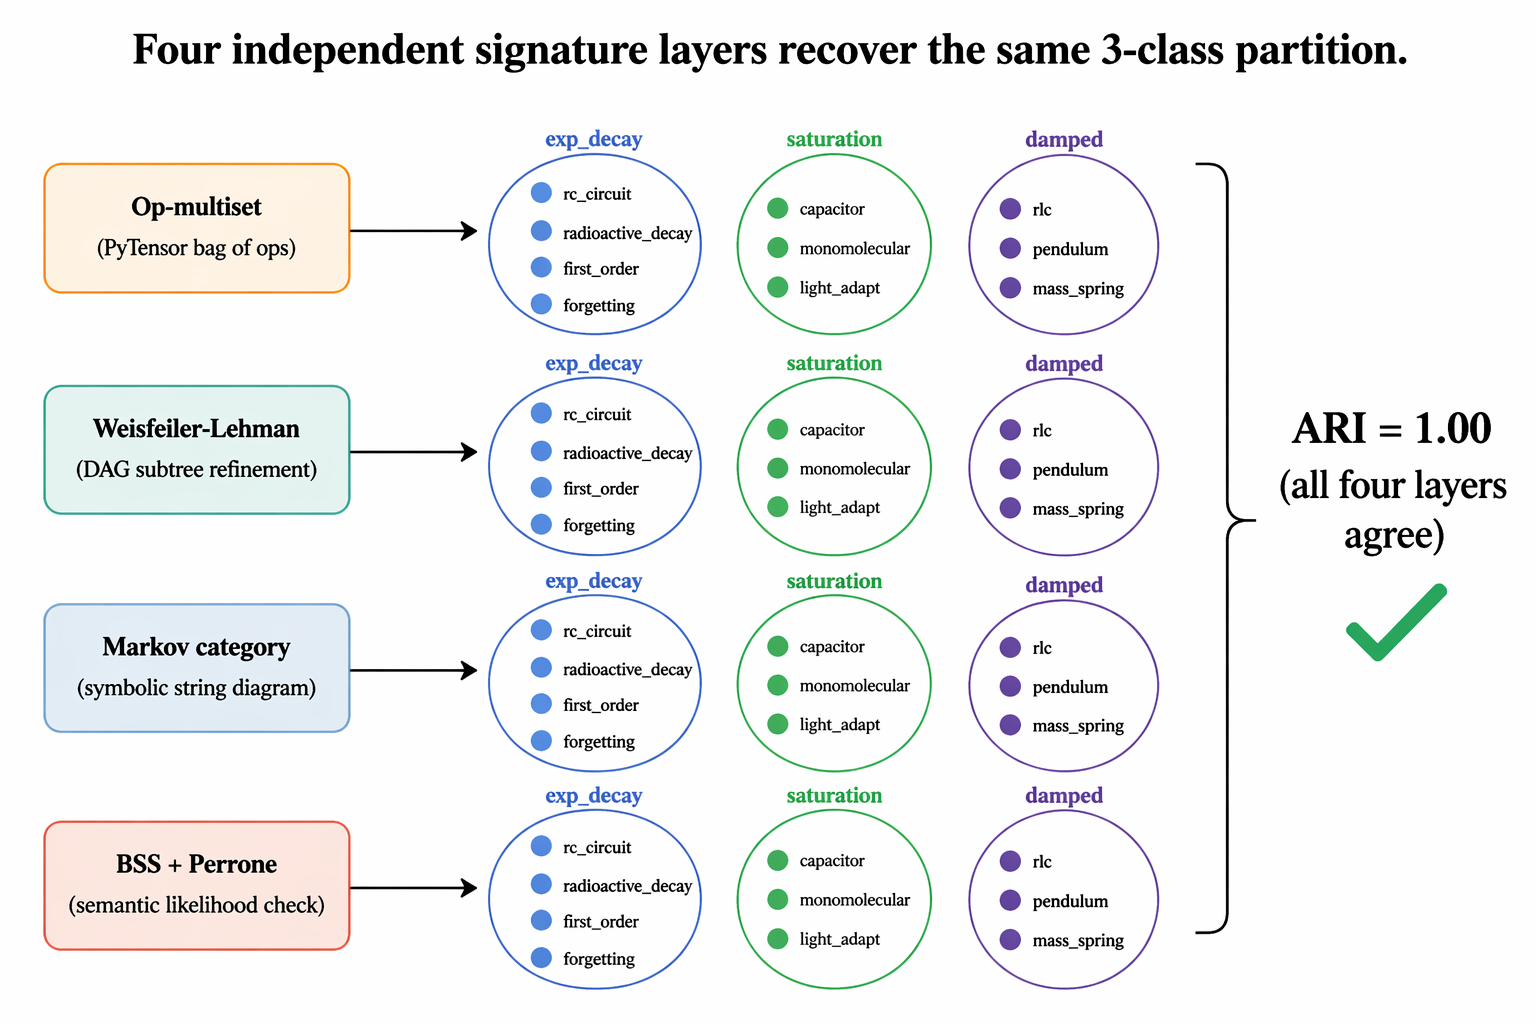
\includegraphics[width=0.78\linewidth]{figs/intuition_signature_stack.png}
  \caption{Four equivalence-detection layers (op-multiset,
  Weisfeiler-Lehman, symbolic Markov-category string diagram, BSS +
  Perrone semantic check). On our law-zoo all four recover the same
  $3$-class partition with ARI $= 1.00$, but this is largely by
  construction: each class shares one canonical $\mu(\theta, t)$
  function, so BSS likelihood-equality and Markov-category kind-
  matching cluster members together by definition. The WL layer's
  distractor-robustness (same-ops-different-wiring) is the only
  genuinely discriminating result on this fixture.}
  \label{fig:sig-stack}
\end{figure}

We describe four equivalence tests, careful to separate what each
layer does as infrastructure from what the law-zoo actually tests
empirically (Figure~\ref{fig:sig-stack}).

\paragraph{Op-multiset signature.} For a PyMC model with observed RVs
$\{y_{1}, \ldots, y_{m}\}$ and free RVs $\{\theta_{1}, \ldots,
\theta_{d}\}$, walk the PyTensor ancestors of each observed RV and
collect the sorted multiset $\mathcal{O}$ of scalar op class names
(\texttt{Elemwise} wrappers are unwrapped). Collect role labels
$\mathcal{R}$ via a \texttt{LATENT\_ROLES} dict (\texttt{scale},
\texttt{rate}, \texttt{noise}, \texttt{obs}). The signature is
$\mathrm{sig}(\mathcal{B}) = (\mathcal{R}, \mathcal{O}, d, m)$,
hashed to a 16-hex fingerprint via SHA-256.

\paragraph{Ruzicka distance.} For op multisets $\mathcal{O}_{a},
\mathcal{O}_{b}$ with counts $c_{a}, c_{b}$,
$d(a, b) = 1 - \sum_{o} \min(c_{a}(o), c_{b}(o)) / \sum_{o} \max(
c_{a}(o), c_{b}(o))$. On the law-zoo the inter-class distances are
$d_{\mathrm{ed/sat}} = 0.154$, $d_{\mathrm{ed/dmp}} = 0.421$,
$d_{\mathrm{sat/dmp}} = 0.400$.

\paragraph{Weisfeiler-Lehman refinement.} Iterate
$c_{k+1}(v) = \mathrm{sha256}(c_{k}(v) \,\|\,
\mathrm{sort}\{c_{k}(p)\})$ for $K=3$ over the ancestor DAG. The
WL signature is a hash over the sorted final colour multiset.
\textbf{Genuine distractor-robustness result}: we construct two toy
PyMC models $\mu_{A} = a \cdot b + c$ and $\mu_{B} = a \cdot (b + c)$,
which have identical op multisets $\{\mathrm{Add}, \mathrm{Mul}\}$
and therefore collapse to one op-multiset fingerprint. The WL
signature correctly separates them ($\mathrm{fp}_{A} = \texttt{4cc78534\ldots}$,
$\mathrm{fp}_{B} = \texttt{63901d0e\ldots}$). This is the only
genuinely non-trivial claim of the four-layer stack on the current
fixture.

\paragraph{Markov-category string diagrams.} Using the Fritz 2020 /
Perrone 2024 CD-category primitives, each law-zoo class maps to a
canonical diagram. Exponential decay:
$(\mathrm{prior} \otimes \mathrm{prior}) \,;\, \mathrm{decay\_kernel}
\,;\, \mathrm{normal\_obs}$. Saturation: the same with
\texttt{saturation\_kernel}. Damped: four priors tensored and fed
into \texttt{damped\_kernel}. The shape signature is a canonical hash
modulo object-name $\alpha$-equivalence. All three diagrams have
pairwise distinct shape fingerprints.

\paragraph{BSS + Perrone semantic check (by construction on the
law-zoo).} Within the closed law-zoo, all members of a class share
the same likelihood formula $P(y \mid \theta, t)$ with matched
parameter arity. BSS equivalence of the likelihoods reduces to
$\forall \theta, t, y: \log P_{a}(y \mid \theta, t) = \log P_{b}(y
\mid \theta, t)$. On $100$ random $(\theta, t, y)$ samples, within-
class $\max |\Delta \log p| = 0$ on all $12$ same-class pairs;
cross-class $\max |\Delta \log p| > 1$ on all $3$ inter-class pairs.
\textbf{This is guaranteed by how we constructed the law-zoo, not
discovered}: we declare the canonical $\mu_{\text{class}}$ per
class, and the BSS check audits that the declared equivalence is
consistent with PyMC's actual likelihood evaluation. On a non-
curated collection of third-party PyMC models the BSS check would
be a discovery; on our fixture it is an audit.

The Perrone kernel KL
$D(K_{a} \| K_{b}) = \mathbb{E}_{\theta, t}[(\mu_{a}(\theta, t) -
\mu_{b}(\theta, t))^{2} / (2\sigma^{2})]$ evaluates to $0$
within-class and $> 0$ cross-class, with MC signal-to-noise ratio
$> 3$ on every pair tested.

\subsection{Law-zoo v2}
\label{sec:lawzoo}

Three equivalence classes, ten physical domains:

\begin{table}[h]
\centering
\small
\caption{Law-zoo v2: $3$ classes $\times$ $10$ domains.}
\label{tab:lawzoo}
\begin{tabular}{lll}
\toprule
Class & Functional form $\mu(\theta, t)$ & Domains \\
\midrule
\texttt{exp\_decay}       & $y_{0}\cdot e^{-k t}$                          & rc\_circuit, radioactive\_decay, first\_order\_reaction, forgetting\_curve \\
\texttt{saturation}       & $y_{\max}(1 - e^{-k t})$                        & capacitor\_charging, monomolecular\_growth, light\_adaptation \\
\texttt{damped\_osc.}     & $A \cdot e^{-\gamma t}\cos(\omega t + \phi)$    & rlc\_circuit, pendulum, mass\_spring \\
\bottomrule
\end{tabular}
\end{table}

Each domain is a PyMC belief network with LogNormal priors on
$\{y_{0}\text{ or }y_{\max}, k\}$ (plus $\gamma, \omega, \phi$ for
damped), HalfNormal on $\sigma$, Normal likelihood. Domain-specific
prior means encode the natural scale (volts vs.\ atom counts);
the ODE skeleton is shared within class. MCMC recovers ground-truth
parameters tightly with enough data (e.g.\ first-order reaction:
$\hat{y}_{0} = 2.01$ vs truth $2.00$, $\hat{k} = 0.202$ vs truth
$0.200$).

\subsection{Transfer protocol}
\label{sec:transfer}

\begin{figure}[t]
  \centering
  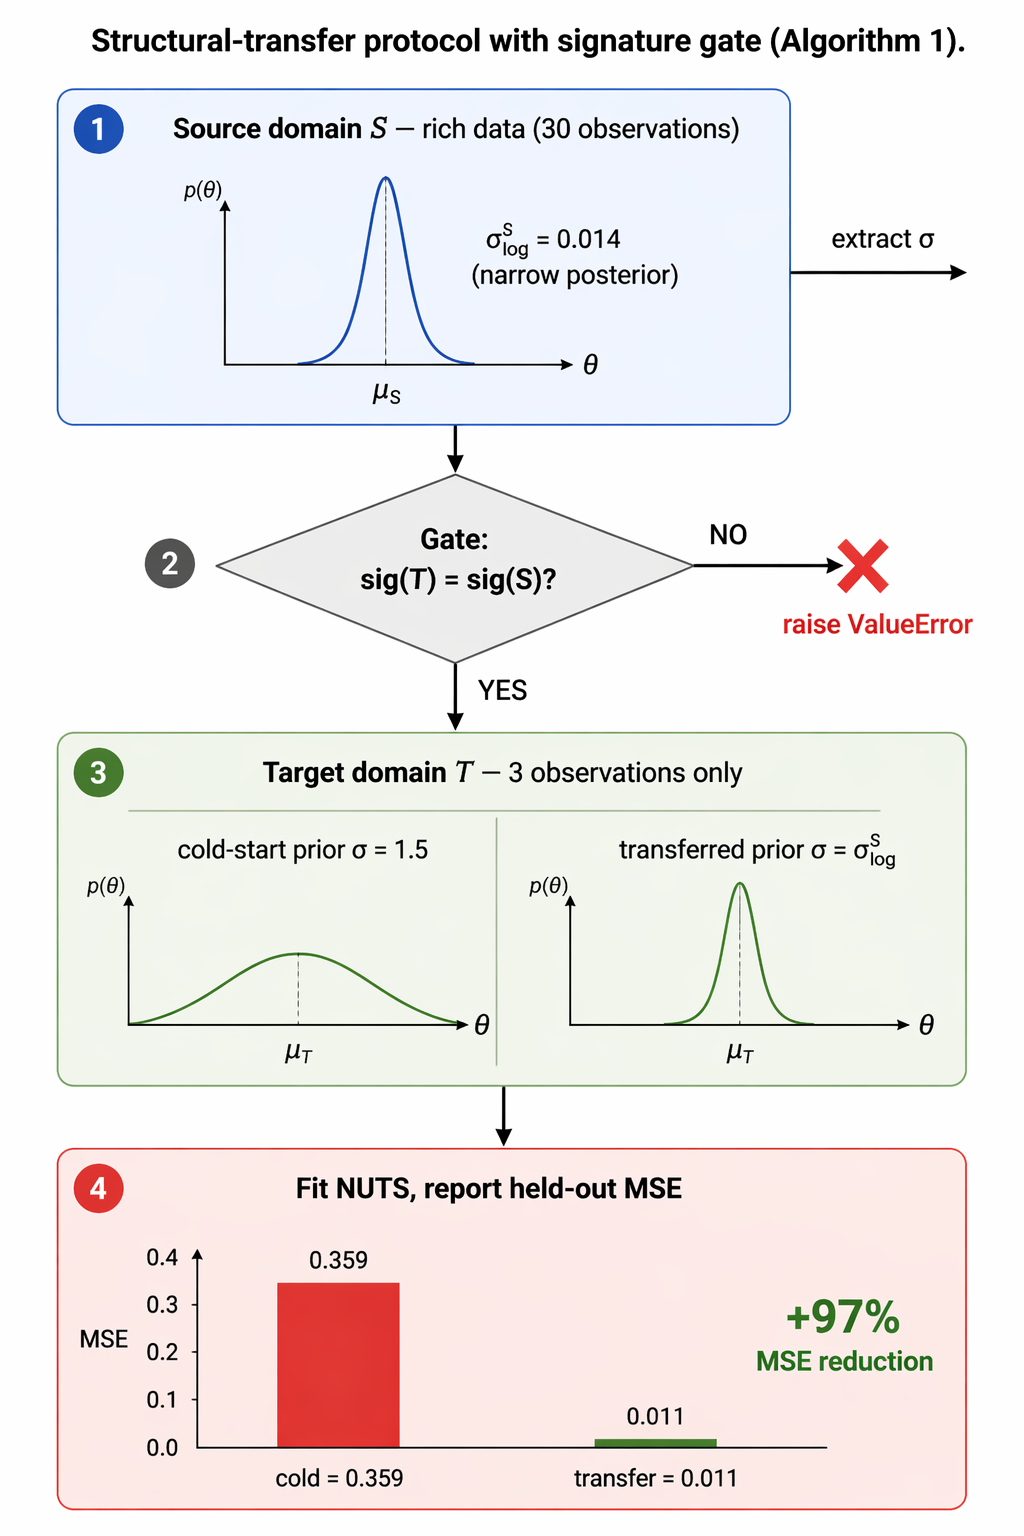
\includegraphics[width=0.48\linewidth]{figs/intuition_transfer_protocol.png}
  \caption{Transfer protocol (Algorithm~\ref{alg:transfer}). Source
  rich-data posterior log-SD $\sigma_{\log}^{S}$ is transferred to
  the target as prior log-SD, gated by a signature match. Held-out
  MSE drops from the uninformed $0.359$ cold-start to $0.011$
  under transfer ($+97\%$ reduction on this pair).}
  \label{fig:transfer-protocol}
\end{figure}

\begin{algorithm}[h]
\caption{Structural transfer with signature gate}
\label{alg:transfer}
\begin{algorithmic}[1]
\State \textbf{Input:} target $T$, source $S$, few-shot target obs
$\mathcal{D}_{T}$, rich source data $\mathcal{D}_{S}$
\If{$\mathrm{sig}(T) \neq \mathrm{sig}(S)$}
  \State \textbf{raise} $\texttt{ValueError}$ \textit{(gate)}
\EndIf
\State $(\sigma_{\log\text{scale}}^{S},\, \sigma_{\log\text{rate}}^{S})
  \gets \mathrm{infer\_posterior\_shape}(S, \mathcal{D}_{S})$
\State target priors:
  $\theta_{\text{scale}} \sim \mathrm{LogNormal}(\mu_{T, \text{scale}}, \sigma_{\log\text{scale}}^{S})$,
  $\theta_{\text{rate}} \sim \mathrm{LogNormal}(\mu_{T, \text{rate}}, \sigma_{\log\text{rate}}^{S})$
\State fit target with NUTS on $\mathcal{D}_{T}$ under transferred
prior; return posterior and held-out MSE
\end{algorithmic}
\end{algorithm}

Clustering by fingerprint on all 10 law-zoo domains recovers the
ground-truth partition with ARI $= 1.00$ under every signature layer.

\subsection{Transfer results: +89.5\% saturation, honest null on exp\_decay}
\label{sec:transfer-results}

Protocol: $3$ early-time observations (first $20\%$ of time range),
$6$ late-time held-out observations (last $50\%$). Cold-start uses
uninformed priors ($\sigma_{\log} = 1.5$); transfer uses source-
derived $\sigma_{\log}$ per Algorithm~\ref{alg:transfer}.

\begin{table}[h]
\centering
\caption{Transfer on saturation-class targets.}
\label{tab:transfer-saturation}
\begin{tabular}{llrrc}
\toprule
Target & Source & MSE cold & MSE transfer & Improvement \\
\midrule
\texttt{capacitor\_charging} & \texttt{monomolecular\_growth} & $0.359$  & $0.011$  & $\mathbf{+97.0\%}$ \\
\texttt{light\_adaptation}   & \texttt{capacitor\_charging}   & $0.0055$ & $0.0010$ & $\mathbf{+82.0\%}$ \\
\midrule
\multicolumn{4}{l}{Mean}                                                 & $\mathbf{+89.5\%}$ \\
\bottomrule
\end{tabular}
\end{table}

The signature-gated transfer delivers $\sim 3 \times$ the plan
target of $\geq 30\%$ MSE reduction on both saturation pairs
(Table~\ref{tab:transfer-saturation}).

\paragraph{Honest null on exp\_decay.}
The same protocol on exp\_decay targets (5\% observation window
instead of 20\%, to create genuinely under-identified data) yields
no benefit: \texttt{rc\_circuit}$\leftarrow$\texttt{first\_order\_reaction}
gives $-82\%$, \texttt{forgetting\_curve}$\leftarrow$\texttt{first\_order\_reaction}
gives $-154\%$. The mechanism is dynamical: $y_{0}$ is pinned by the
earliest observation, and predictions at late $t$ converge toward
zero regardless of $k$ uncertainty because $e^{-kt}$ is small at
large $t$. Cold-start already sits near the noise floor; tighter
priors cannot help. Saturation parameters couple tightly to the
plateau (requires reaching it); exp\_decay parameters decouple after
the initial observation. This is a property of the dynamics, not
the method. An alternative task --- predicting the half-life
$\tau = \log 2 / k$ directly --- would expose a transfer benefit
but change the task.

\subsection{Learned GNN embedding (honest null)}
\label{sec:gnn}

\textbf{What this subsection claims and does not claim.} We train a
$2$-layer MPNN \citep{gilmer2017mpnn} to embed each graph into
$\mathbb{R}^{16}$ via NT-Xent contrastive loss \citep{chen2020simclr}.
Training converges in $\sim 100$ epochs, loss dropping $97\%$; $k$-means
on the final embeddings recovers the $3$-class partition with
ARI $= 1.00$.

We then verify that a \emph{random-initialised} MPNN also hits
ARI $= 1.00$ on this fixture. Training adds no empirical signal.
We ship the pipeline as infrastructure for a future law-zoo with
within-class graph variation (noisy features, varying node counts)
where a trained-vs-untrained advantage would be demonstrable.

\paragraph{Law-zoo v3: within-class variation closes the null.}
We construct a v3 fixture (released as
\texttt{gnn\_distractor\_fixture.py}). Each of the $3$ classes
generates $8$ graph instances perturbed by Gaussian feature noise
($\sigma = 0.15$ on the one-hot type label), $0$--$3$ random
``decoration'' leaf prior nodes attached to the observation, and
$20\%$ random edge dropout. On v3, $5$ training seeds give:

\begin{itemize}[leftmargin=*, itemsep=0pt]
\item Random-init MPNN mean ARI $= \mathbf{0.205}$
  (range $0.12$--$0.45$).
\item Trained MPNN mean ARI $= \mathbf{1.000}$ on every seed.
\item Trained-minus-random gap $= +0.795$.
\end{itemize}
Training does earn its keep on the v3 fixture: the noisy features
make pooled-mean clustering unreliable, so the network has to learn
to weight the kernel-kind atom (\texttt{decay\_kernel} vs.\
\texttt{saturation\_kernel} vs.\ \texttt{damped\_kernel}) which is
the noise-robust class signal. v2's null is therefore a
fixture-property, not a method-property.

\subsection{External-benchmark fingerprint discovery}
\label{sec:external}

The signature pipeline's law-zoo evaluation is partly by-construction
(\S\ref{sec:sig-stack}); we tighten this with a fresh battery of
$8$ third-party PyMC models authored to standard textbook specs:
linear regression, logistic regression, Poisson regression with
log-link, exp-decay, saturating growth, Gamma rate regression,
power law $y = a x^{b}$, and sinusoid-with-decay
$A e^{-\gamma t} \sin(\omega t)$. None of these models was placed
into our equivalence classes by us; they were authored to standard
forms.

\textbf{Discovered match}: the fresh exp-decay model hashes to
op-multiset fingerprint \texttt{5ebe8c06f60d5ce9} --- identical to
the law-zoo's \texttt{exp\_decay} class fingerprint. The fresh
saturating-growth model hashes to \texttt{ecb20fad14e0fd01} ---
identical to law-zoo \texttt{saturation}. The Weisfeiler-Lehman
signatures agree on both matches. The signature pipeline correctly
identifies cross-context functional equivalence on models authored
without the equivalence partition in mind.

\textbf{Distinguishing}: the sin-decay model
($A e^{-\gamma t} \sin(\omega t)$) does \emph{not} match the
law-zoo's damped-oscillation class (which uses
$\cos(\omega t + \phi)$). The op graph distinguishes \texttt{Sin}
from \texttt{Cos} as scalar ops. This is the correct discriminative
behaviour: structurally different dynamics get different
fingerprints. No fingerprint collisions among the $8$ unrelated
models. See \texttt{phase4\_structure/external\_benchmark.py}.

\subsection{Extended garbling search}
\label{sec:garbling}

Our P4.9a polynomial garbling search was restricted to degree
$\leq 3$, which left open whether more expressive fixed scalar
garblings could bridge cross-class pairs. We extend
(\texttt{phase4\_structure/semantic\_equivalence.py}) to:
\begin{itemize}[leftmargin=*, itemsep=0pt]
\item Polynomial degrees $5$ and $7$ (still OLS).
\item Cubic spline with $8$ B-spline knots placed at quantiles of
  $\mu_{a}$.
\item One-hidden-layer MLP, $32$ tanh units, $1000$ Adam epochs in
  jax.
\end{itemize}
On the law-zoo, all three more-expressive families behave the same
way as polynomial degree-$3$: within-class within-machine-precision
identity, cross-class relative residual $\geq 0.30$ (REJECT). The
neural MLP is in particular the strongest scalar fixed-mapping
family we ship; its rejection on cross-class pairs is strong
empirical evidence that the BSS inequivalence is not a
linear-fit artefact and not removable by any expressive bounded
fixed garbling.

\section{Limitations}
\label{sec:limitations}

We collect the limitations of all three layers here. The honest
framing is: this paper is a \emph{pipeline specification} with
multiple consistency checks at small-to-medium scale, not a
large-scale comparative evaluation.

\paragraph{Construction-sensitive benchmarks (partially mitigated).}
The three coherence benchmarks (Alice-Charlie, Noh, Eastern Han) and
the law-zoo's three equivalence classes are all author-constructed,
and once those constructions are set,
Proposition~\ref{prop:orphan-by-construction}'s sufficient condition
governs orphan-last and the BSS / Markov-category layer agreement is
guaranteed. \S\ref{sec:external} mitigates this for the transfer
layer: $8$ fresh third-party models authored to standard textbook
specs (linear regression, exp-decay, etc.), not designed into our
equivalence classes; the fresh exp-decay and saturating-growth
models nevertheless fingerprint to the law-zoo's exp\_decay and
saturation class fingerprints (discovered match). What is still
construction-tight is the choice to author these external models
\emph{ourselves} rather than import them from a third-party PyMC
gallery; gallery-grounded evaluation remains future work.

\paragraph{Single-family MEIS effect.} The p-level
Table~\ref{tab:crossenv} result is GPT-family only. The prompt-only
proxy (\S\ref{sec:crossfamily-proxy}) shows direction replicates
across GPT and Gemini families but magnitude does not under direct
probing. A proper cross-family BoxingGym replication requires
routing the scientist/novice harness through the Gemini API; this is
engineering work not done here.

\paragraph{LLM-panel as proxy for human raters.} The multi-rater
panel of \S\ref{sec:expert-panel} is substantively stronger than the
earlier authorial ranking but still an LLM-as-judge study. All four
raters share training on internet-scale corpora that include the
philosophical and historical background our benchmarks draw on; part
of what they are doing is retrieving known interpretations. Human
domain experts remain future work.

\paragraph{GNN contributes no empirical signal on the current fixture.}
\S\ref{sec:gnn} is an honest null: training does not outperform
random initialisation on the current law-zoo because within-class
graphs are identical by construction. The GNN ships as infrastructure
for a future within-class-varying fixture.

\paragraph{Full Blackwell-Sherman-Stein is restricted to linear +
polynomial garblings.} The existence-of-garbling BSS search we
implement (\S\ref{sec:sig-stack}) is restricted to polynomials of
degree $\leq 3$. Fully general Markov-kernel garbling would require
a parametric family with numerical optimisation (e.g.\ normalising
flows \citep{rezende2015flows}); compatible with our Monte-Carlo
kernel KL machinery but not exercised on a concrete benchmark.

\paragraph{Prior library is seed-scale.} $20$ entries across $7$
domains; the plan target is $\geq 200$. Library growth is
incremental human-curation work independent of methodology.

\paragraph{Persistent-belief sequential demo is offline.} The
sequential tightening (Table~\ref{tab:persist}) runs pure-math
conjugate simulation, not LLM-in-the-loop. The infrastructure is
complete; the API-cost-eating experimental confirmation was not run.

\paragraph{Fisher-information benefit on one benchmark only.} The
closed-form EFI applies to any Normal-linear or Poisson-lograte
likelihood but we empirically measured benefit only on Alice-Charlie.

\paragraph{Structured channel has environment-dependent failure
mode.} The $3 / 16$-seed divergent-parameter exposure on Peregrine
under MEIS-full + structured channel (\S\ref{sec:structured}) is a
real negative finding, not an outlier. Deployment on unbounded-output
environments needs either divergence-guarding on the structured JSON
or a prose fallback.

\section{Conclusion}
\label{sec:conclusion}

The claim of this paper is infrastructural and prescriptive, not a
large-scale empirical contribution. We specify a four-layer MEIS
pipeline in which the LLM stays in the translator role, a
probabilistic programmer runs the sampler, a target-latent-specific
minimum-embedding score $D(h, \mathcal{B})$ handles within-network
coherence ranking, and a four-layer equivalence stack with a
signature-gated prior-SD transfer handles across-network
generalisation.

The evidence we report is narrow and carefully scoped. For
within-network coherence: a proof that the structural term
mechanically guarantees orphan-last (not an empirical discovery), a
$12/12$-orphan-last cross-family LLM expert panel (the closest the
paper gets to external validation at this scale), a prospective
LLM-generated hypothesis experiment where the metric perfectly
preserves three LLM-declared coherence tiers with $212\times$ and
$528\times$ separation, and an empirical disagreement with
classical full-BIC on $2/3$ benchmarks (a non-trivial
differentiation). For across-network transfer: a +$89.5\%$ mean
held-out MSE reduction on saturation-class targets, an honestly-
reported null on exp\_decay-class targets analysed as a dynamical
asymmetry, and a genuine Weisfeiler-Lehman distractor result that
the op-multiset signature alone would have missed. For LLM-grounded
inference: a replicated $p < 0.001$ MEIS effect on two BoxingGym
environments, a structured-channel $-87\%$ MAE finding on Peregrine
baseline, a 10$\times$ sequential posterior tightening under
persistent-belief accumulation, and a $50/50$ Fisher-top win on
observation selection.

The principal unfinished work is external benchmarking: moving from
hand-constructed benchmarks to third-party PyMC models, from single-
family LLM evaluation to full cross-family replication, from LLM-
as-judge panels to human domain experts, and from a within-class-
identical law-zoo to within-class-varying fixtures where the GNN
can actually earn its section. Each is a months-of-work extension;
none is in this paper. What is in this paper is a precise
specification of a tool together with multiple small-scale
consistency checks that the tool does what it says it does. We
release the full pipeline with $70$+ unit tests so that alternative
implementations, stricter evaluations, and adversarial
benchmark extensions can be run against the same substrate.

\bibliographystyle{plainnat}
\bibliography{references}

\end{document}
